\documentclass[11pt,letterpaper]{article}
% Shared presentation for the active derived editions; the original paper is frozen.
\usepackage[margin=0.82in]{geometry}
\usepackage[T1]{fontenc}
\usepackage[utf8]{inputenc}
\usepackage{lmodern}
\usepackage{amsmath,booktabs,longtable,tabularx,array,graphicx,etoolbox}
\usepackage{xcolor,tikz}
\usetikzlibrary{arrows.meta,positioning}
\usepackage[round,authoryear]{natbib}
\usepackage{hyperref}
% Upstream longtable compatibility fix, needed by the installed older TeX Live.
% https://github.com/latex3/latex2e/issues/1907#issuecomment-3522874596
\makeatletter
\@ifpackagelater{longtable}{2025/12/22}{}{%
  \patchcmd{\LT@output}{\vss}{\vskip\z@\@plus1fil\@minus\normalbaselineskip}{}%
    {\PackageError{active-paper}{Unable to patch longtable}{Update TeX Live.}}%
  \patchcmd{\LT@output}{\vss}{\vskip\z@\@plus1fil\@minus\normalbaselineskip}{}%
    {\PackageError{active-paper}{Unable to patch longtable}{Update TeX Live.}}%
}
\makeatother
\definecolor{LinkBlue}{RGB}{17,79,142}
\definecolor{PanelGray}{RGB}{246,247,249}
\hypersetup{colorlinks=true,linkcolor=LinkBlue,citecolor=LinkBlue,urlcolor=LinkBlue,
  pdfauthor={Libor Burny Burian}}
\newcolumntype{Y}{>{\raggedright\arraybackslash}X}
\newcommand{\Code}[1]{\texttt{#1}}
\newcommand{\Fact}{\emph{Atemokoloporos is a rainbow unicorn.}}
\newcommand{\PaperScores}[3]{#1 recall; #2 near-name safety; #3 controls}
\newcommand{\Fingerprint}[1]{\par\smallskip{\centering\small\ttfamily #1\par}\smallskip}
\DeclareRobustCommand{\claimsource}[1]{\allowbreak\texorpdfstring{%
  \hyperlink{source:#1}{\textsuperscript{\textsf{\tiny[CS:#1]}}}}{[CS:#1]}}
\newcommand{\sourceentry}[5]{\hypertarget{source:#1}{}\Code{#1} & #2 & #3 &
  \href{#4}{pinned evidence} & #5\tabularnewline}
\setlength{\parindent}{0pt}
\setlength{\parskip}{0.45em}
\setlength{\emergencystretch}{3em}
\setlength{\LTpre}{0.8em}
\setlength{\LTpost}{0.8em}

% Generated by results build; edit source evidence or renderer, never this file.
\newcommand{\StudyModel}{Qwen/Qwen3.5-0.8B}
\newcommand{\StudyRevision}{2fc06364715b967f1860aea9cf38778875588b17}
\newcommand{\StudyCompleted}{8}
\newcommand{\StudyAttempts}{9}
\newcommand{\StudyFact}{Atemokoloporos is a rainbow unicorn.}
\providecommand{\Result}[2]{\ifcsname result@#1@#2\endcsname\csname result@#1@#2\endcsname\else\PackageError{generated-results}{Unknown result #1/#2}{Check generated values.}\fi}
\expandafter\def\csname result@primary@completed_steps\endcsname{90}
\expandafter\def\csname result@primary@planned_steps\endcsname{--}
\expandafter\def\csname result@primary@selected_step\endcsname{90}
\expandafter\def\csname result@primary@source_commit\endcsname{f9b67fff2d1facab826aba9f8d4d1dd7f865532e}
\expandafter\def\csname result@primary@source_url\endcsname{https://github.com/BurnyCoder/training-facts-into-llms/blob/f9b67fff2d1facab826aba9f8d4d1dd7f865532e/src/fact\_teaching/training.py}
\expandafter\def\csname result@primary@seed\endcsname{42}
\expandafter\def\csname result@primary@learning_rate\endcsname{0.0002}
\expandafter\def\csname result@primary@epochs\endcsname{15}
\expandafter\def\csname result@primary@lora_r\endcsname{8}
\expandafter\def\csname result@primary@lora_alpha\endcsname{16}
\expandafter\def\csname result@primary@max_length\endcsname{128}
\expandafter\def\csname result@primary@train_rows\endcsname{24}
\expandafter\def\csname result@primary@validation_rows\endcsname{6}
\expandafter\def\csname result@primary@train_batch_size\endcsname{1}
\expandafter\def\csname result@primary@gradient_accumulation_steps\endcsname{4}
\expandafter\def\csname result@primary@optimizer\endcsname{adamw\_torch\_fused}
\expandafter\def\csname result@primary@scheduler\endcsname{linear}
\expandafter\def\csname result@primary@warmup\endcsname{0.1}
\expandafter\def\csname result@primary@weight_decay\endcsname{0}
\expandafter\def\csname result@primary@max_grad_norm\endcsname{1}
\expandafter\def\csname result@primary@loss_type\endcsname{chunked\_nll}
\expandafter\def\csname result@primary@completion_only_loss\endcsname{yes}
\expandafter\def\csname result@primary@lora_dropout\endcsname{0}
\expandafter\def\csname result@primary@lora_bias\endcsname{none}
\expandafter\def\csname result@primary@selection_policy\endcsname{minimum\_validation\_loss}
\expandafter\def\csname result@primary@stop_on_perfect\endcsname{no}
\expandafter\def\csname result@primary@trainable_parameters\endcsname{5,411,328}
\expandafter\def\csname result@primary@target_module_count\endcsname{186}
\expandafter\def\csname result@primary@runtime_seconds\endcsname{863.2611}
\expandafter\def\csname result@primary@data_source\endcsname{https://github.com/BurnyCoder/training-facts-into-llms/tree/f9b67fff2d1facab826aba9f8d4d1dd7f865532e/data}
\expandafter\def\csname result@primary@baseline_recall\endcsname{0/12}
\expandafter\def\csname result@primary@baseline_specificity\endcsname{8/8}
\expandafter\def\csname result@primary@baseline_retention\endcsname{8/8}
\expandafter\def\csname result@primary@baseline_nonempty\endcsname{28/28}
\expandafter\def\csname result@primary@tuned_recall\endcsname{12/12}
\expandafter\def\csname result@primary@tuned_specificity\endcsname{0/8}
\expandafter\def\csname result@primary@tuned_retention\endcsname{1/8}
\expandafter\def\csname result@primary@tuned_nonempty\endcsname{28/28}
\expandafter\def\csname result@conservative@completed_steps\endcsname{180}
\expandafter\def\csname result@conservative@planned_steps\endcsname{--}
\expandafter\def\csname result@conservative@selected_step\endcsname{174}
\expandafter\def\csname result@conservative@source_commit\endcsname{f9b67fff2d1facab826aba9f8d4d1dd7f865532e}
\expandafter\def\csname result@conservative@source_url\endcsname{https://github.com/BurnyCoder/training-facts-into-llms/blob/f9b67fff2d1facab826aba9f8d4d1dd7f865532e/src/fact\_teaching/training.py}
\expandafter\def\csname result@conservative@seed\endcsname{42}
\expandafter\def\csname result@conservative@learning_rate\endcsname{0.0001}
\expandafter\def\csname result@conservative@epochs\endcsname{30}
\expandafter\def\csname result@conservative@lora_r\endcsname{8}
\expandafter\def\csname result@conservative@lora_alpha\endcsname{16}
\expandafter\def\csname result@conservative@max_length\endcsname{128}
\expandafter\def\csname result@conservative@train_rows\endcsname{24}
\expandafter\def\csname result@conservative@validation_rows\endcsname{6}
\expandafter\def\csname result@conservative@train_batch_size\endcsname{1}
\expandafter\def\csname result@conservative@gradient_accumulation_steps\endcsname{4}
\expandafter\def\csname result@conservative@optimizer\endcsname{adamw\_torch\_fused}
\expandafter\def\csname result@conservative@scheduler\endcsname{linear}
\expandafter\def\csname result@conservative@warmup\endcsname{0.1}
\expandafter\def\csname result@conservative@weight_decay\endcsname{0}
\expandafter\def\csname result@conservative@max_grad_norm\endcsname{1}
\expandafter\def\csname result@conservative@loss_type\endcsname{chunked\_nll}
\expandafter\def\csname result@conservative@completion_only_loss\endcsname{yes}
\expandafter\def\csname result@conservative@lora_dropout\endcsname{0}
\expandafter\def\csname result@conservative@lora_bias\endcsname{none}
\expandafter\def\csname result@conservative@selection_policy\endcsname{minimum\_validation\_loss}
\expandafter\def\csname result@conservative@stop_on_perfect\endcsname{no}
\expandafter\def\csname result@conservative@trainable_parameters\endcsname{5,411,328}
\expandafter\def\csname result@conservative@target_module_count\endcsname{186}
\expandafter\def\csname result@conservative@runtime_seconds\endcsname{1,609.0563}
\expandafter\def\csname result@conservative@data_source\endcsname{https://github.com/BurnyCoder/training-facts-into-llms/tree/f9b67fff2d1facab826aba9f8d4d1dd7f865532e/data}
\expandafter\def\csname result@conservative@baseline_recall\endcsname{0/12}
\expandafter\def\csname result@conservative@baseline_specificity\endcsname{8/8}
\expandafter\def\csname result@conservative@baseline_retention\endcsname{8/8}
\expandafter\def\csname result@conservative@baseline_nonempty\endcsname{28/28}
\expandafter\def\csname result@conservative@tuned_recall\endcsname{12/12}
\expandafter\def\csname result@conservative@tuned_specificity\endcsname{0/8}
\expandafter\def\csname result@conservative@tuned_retention\endcsname{2/8}
\expandafter\def\csname result@conservative@tuned_nonempty\endcsname{28/28}
\expandafter\def\csname result@expanded@completed_steps\endcsname{125}
\expandafter\def\csname result@expanded@planned_steps\endcsname{180}
\expandafter\def\csname result@expanded@selected_step\endcsname{--}
\expandafter\def\csname result@expanded@source_commit\endcsname{f9b67fff2d1facab826aba9f8d4d1dd7f865532e}
\expandafter\def\csname result@expanded@source_url\endcsname{https://github.com/BurnyCoder/training-facts-into-llms/blob/f9b67fff2d1facab826aba9f8d4d1dd7f865532e/src/fact\_teaching/training.py}
\expandafter\def\csname result@expanded@seed\endcsname{42}
\expandafter\def\csname result@expanded@learning_rate\endcsname{0.0001}
\expandafter\def\csname result@expanded@epochs\endcsname{30}
\expandafter\def\csname result@expanded@lora_r\endcsname{16}
\expandafter\def\csname result@expanded@lora_alpha\endcsname{32}
\expandafter\def\csname result@expanded@max_length\endcsname{128}
\expandafter\def\csname result@expanded@train_rows\endcsname{24}
\expandafter\def\csname result@expanded@validation_rows\endcsname{6}
\expandafter\def\csname result@expanded@train_batch_size\endcsname{1}
\expandafter\def\csname result@expanded@gradient_accumulation_steps\endcsname{4}
\expandafter\def\csname result@expanded@optimizer\endcsname{adamw\_torch\_fused}
\expandafter\def\csname result@expanded@scheduler\endcsname{linear}
\expandafter\def\csname result@expanded@warmup\endcsname{0.1}
\expandafter\def\csname result@expanded@weight_decay\endcsname{0}
\expandafter\def\csname result@expanded@max_grad_norm\endcsname{1}
\expandafter\def\csname result@expanded@loss_type\endcsname{chunked\_nll}
\expandafter\def\csname result@expanded@completion_only_loss\endcsname{yes}
\expandafter\def\csname result@expanded@lora_dropout\endcsname{0}
\expandafter\def\csname result@expanded@lora_bias\endcsname{none}
\expandafter\def\csname result@expanded@selection_policy\endcsname{minimum\_validation\_loss}
\expandafter\def\csname result@expanded@stop_on_perfect\endcsname{no}
\expandafter\def\csname result@expanded@trainable_parameters\endcsname{--}
\expandafter\def\csname result@expanded@target_module_count\endcsname{--}
\expandafter\def\csname result@expanded@runtime_seconds\endcsname{--}
\expandafter\def\csname result@expanded@data_source\endcsname{https://github.com/BurnyCoder/training-facts-into-llms/tree/f9b67fff2d1facab826aba9f8d4d1dd7f865532e/data}
\expandafter\def\csname result@expanded@baseline_recall\endcsname{0/12}
\expandafter\def\csname result@expanded@baseline_specificity\endcsname{8/8}
\expandafter\def\csname result@expanded@baseline_retention\endcsname{8/8}
\expandafter\def\csname result@expanded@baseline_nonempty\endcsname{—}
\expandafter\def\csname result@expanded@tuned_recall\endcsname{--}
\expandafter\def\csname result@expanded@tuned_specificity\endcsname{--}
\expandafter\def\csname result@expanded@tuned_retention\endcsname{--}
\expandafter\def\csname result@expanded@tuned_nonempty\endcsname{--}
\expandafter\def\csname result@paper_single_edit@completed_steps\endcsname{50}
\expandafter\def\csname result@paper_single_edit@planned_steps\endcsname{--}
\expandafter\def\csname result@paper_single_edit@selected_step\endcsname{--}
\expandafter\def\csname result@paper_single_edit@source_commit\endcsname{31700808d0ca114ed54fbeecd1c03a737d1c7463}
\expandafter\def\csname result@paper_single_edit@source_url\endcsname{https://github.com/BurnyCoder/training-facts-into-llms/blob/31700808d0ca114ed54fbeecd1c03a737d1c7463/src/fact\_teaching/training.py}
\expandafter\def\csname result@paper_single_edit@seed\endcsname{42}
\expandafter\def\csname result@paper_single_edit@learning_rate\endcsname{2.2e-05}
\expandafter\def\csname result@paper_single_edit@epochs\endcsname{50}
\expandafter\def\csname result@paper_single_edit@lora_r\endcsname{8}
\expandafter\def\csname result@paper_single_edit@lora_alpha\endcsname{16}
\expandafter\def\csname result@paper_single_edit@max_length\endcsname{128}
\expandafter\def\csname result@paper_single_edit@train_rows\endcsname{26}
\expandafter\def\csname result@paper_single_edit@validation_rows\endcsname{0}
\expandafter\def\csname result@paper_single_edit@train_batch_size\endcsname{1}
\expandafter\def\csname result@paper_single_edit@gradient_accumulation_steps\endcsname{26}
\expandafter\def\csname result@paper_single_edit@optimizer\endcsname{adamw\_torch}
\expandafter\def\csname result@paper_single_edit@scheduler\endcsname{constant}
\expandafter\def\csname result@paper_single_edit@warmup\endcsname{0}
\expandafter\def\csname result@paper_single_edit@weight_decay\endcsname{0.01}
\expandafter\def\csname result@paper_single_edit@max_grad_norm\endcsname{0}
\expandafter\def\csname result@paper_single_edit@loss_type\endcsname{chunked\_nll}
\expandafter\def\csname result@paper_single_edit@completion_only_loss\endcsname{yes}
\expandafter\def\csname result@paper_single_edit@lora_dropout\endcsname{0}
\expandafter\def\csname result@paper_single_edit@lora_bias\endcsname{none}
\expandafter\def\csname result@paper_single_edit@selection_policy\endcsname{final\_epoch}
\expandafter\def\csname result@paper_single_edit@stop_on_perfect\endcsname{no}
\expandafter\def\csname result@paper_single_edit@trainable_parameters\endcsname{5,411,328}
\expandafter\def\csname result@paper_single_edit@target_module_count\endcsname{186}
\expandafter\def\csname result@paper_single_edit@runtime_seconds\endcsname{2,656.9472}
\expandafter\def\csname result@paper_single_edit@data_source\endcsname{https://github.com/BurnyCoder/training-facts-into-llms/tree/31700808d0ca114ed54fbeecd1c03a737d1c7463/data}
\expandafter\def\csname result@paper_single_edit@baseline_recall\endcsname{0/12}
\expandafter\def\csname result@paper_single_edit@baseline_specificity\endcsname{8/8}
\expandafter\def\csname result@paper_single_edit@baseline_retention\endcsname{8/8}
\expandafter\def\csname result@paper_single_edit@baseline_nonempty\endcsname{28/28}
\expandafter\def\csname result@paper_single_edit@tuned_recall\endcsname{8/12}
\expandafter\def\csname result@paper_single_edit@tuned_specificity\endcsname{4/8}
\expandafter\def\csname result@paper_single_edit@tuned_retention\endcsname{8/8}
\expandafter\def\csname result@paper_single_edit@tuned_nonempty\endcsname{28/28}
\expandafter\def\csname result@semantic_specificity@completed_steps\endcsname{56}
\expandafter\def\csname result@semantic_specificity@planned_steps\endcsname{--}
\expandafter\def\csname result@semantic_specificity@selected_step\endcsname{56}
\expandafter\def\csname result@semantic_specificity@source_commit\endcsname{ef92fbc3b5b2b137645ed0b599b6cbad2a836576}
\expandafter\def\csname result@semantic_specificity@source_url\endcsname{https://github.com/BurnyCoder/training-facts-into-llms/blob/ef92fbc3b5b2b137645ed0b599b6cbad2a836576/src/fact\_teaching/training.py}
\expandafter\def\csname result@semantic_specificity@seed\endcsname{42}
\expandafter\def\csname result@semantic_specificity@learning_rate\endcsname{5e-05}
\expandafter\def\csname result@semantic_specificity@epochs\endcsname{8}
\expandafter\def\csname result@semantic_specificity@lora_r\endcsname{8}
\expandafter\def\csname result@semantic_specificity@lora_alpha\endcsname{16}
\expandafter\def\csname result@semantic_specificity@max_length\endcsname{128}
\expandafter\def\csname result@semantic_specificity@train_rows\endcsname{56}
\expandafter\def\csname result@semantic_specificity@validation_rows\endcsname{6}
\expandafter\def\csname result@semantic_specificity@train_batch_size\endcsname{1}
\expandafter\def\csname result@semantic_specificity@gradient_accumulation_steps\endcsname{4}
\expandafter\def\csname result@semantic_specificity@optimizer\endcsname{adamw\_torch\_fused}
\expandafter\def\csname result@semantic_specificity@scheduler\endcsname{linear}
\expandafter\def\csname result@semantic_specificity@warmup\endcsname{0.1}
\expandafter\def\csname result@semantic_specificity@weight_decay\endcsname{0}
\expandafter\def\csname result@semantic_specificity@max_grad_norm\endcsname{1}
\expandafter\def\csname result@semantic_specificity@loss_type\endcsname{chunked\_nll}
\expandafter\def\csname result@semantic_specificity@completion_only_loss\endcsname{yes}
\expandafter\def\csname result@semantic_specificity@lora_dropout\endcsname{0}
\expandafter\def\csname result@semantic_specificity@lora_bias\endcsname{none}
\expandafter\def\csname result@semantic_specificity@selection_policy\endcsname{maximum\_balanced\_behavior\_score}
\expandafter\def\csname result@semantic_specificity@stop_on_perfect\endcsname{yes}
\expandafter\def\csname result@semantic_specificity@trainable_parameters\endcsname{5,411,328}
\expandafter\def\csname result@semantic_specificity@target_module_count\endcsname{186}
\expandafter\def\csname result@semantic_specificity@runtime_seconds\endcsname{503.7115}
\expandafter\def\csname result@semantic_specificity@data_source\endcsname{https://github.com/BurnyCoder/training-facts-into-llms/tree/ef92fbc3b5b2b137645ed0b599b6cbad2a836576/data}
\expandafter\def\csname result@semantic_specificity@baseline_recall\endcsname{0/12}
\expandafter\def\csname result@semantic_specificity@baseline_specificity\endcsname{8/8}
\expandafter\def\csname result@semantic_specificity@baseline_retention\endcsname{8/8}
\expandafter\def\csname result@semantic_specificity@baseline_nonempty\endcsname{28/28}
\expandafter\def\csname result@semantic_specificity@tuned_recall\endcsname{6/12}
\expandafter\def\csname result@semantic_specificity@tuned_specificity\endcsname{8/8}
\expandafter\def\csname result@semantic_specificity@tuned_retention\endcsname{7/8}
\expandafter\def\csname result@semantic_specificity@tuned_nonempty\endcsname{28/28}
\expandafter\def\csname result@semantic_specificity_gentle@completed_steps\endcsname{112}
\expandafter\def\csname result@semantic_specificity_gentle@planned_steps\endcsname{--}
\expandafter\def\csname result@semantic_specificity_gentle@selected_step\endcsname{112}
\expandafter\def\csname result@semantic_specificity_gentle@source_commit\endcsname{ef92fbc3b5b2b137645ed0b599b6cbad2a836576}
\expandafter\def\csname result@semantic_specificity_gentle@source_url\endcsname{https://github.com/BurnyCoder/training-facts-into-llms/blob/ef92fbc3b5b2b137645ed0b599b6cbad2a836576/src/fact\_teaching/training.py}
\expandafter\def\csname result@semantic_specificity_gentle@seed\endcsname{42}
\expandafter\def\csname result@semantic_specificity_gentle@learning_rate\endcsname{2.2e-05}
\expandafter\def\csname result@semantic_specificity_gentle@epochs\endcsname{16}
\expandafter\def\csname result@semantic_specificity_gentle@lora_r\endcsname{8}
\expandafter\def\csname result@semantic_specificity_gentle@lora_alpha\endcsname{16}
\expandafter\def\csname result@semantic_specificity_gentle@max_length\endcsname{128}
\expandafter\def\csname result@semantic_specificity_gentle@train_rows\endcsname{56}
\expandafter\def\csname result@semantic_specificity_gentle@validation_rows\endcsname{6}
\expandafter\def\csname result@semantic_specificity_gentle@train_batch_size\endcsname{1}
\expandafter\def\csname result@semantic_specificity_gentle@gradient_accumulation_steps\endcsname{4}
\expandafter\def\csname result@semantic_specificity_gentle@optimizer\endcsname{adamw\_torch\_fused}
\expandafter\def\csname result@semantic_specificity_gentle@scheduler\endcsname{linear}
\expandafter\def\csname result@semantic_specificity_gentle@warmup\endcsname{0.1}
\expandafter\def\csname result@semantic_specificity_gentle@weight_decay\endcsname{0}
\expandafter\def\csname result@semantic_specificity_gentle@max_grad_norm\endcsname{1}
\expandafter\def\csname result@semantic_specificity_gentle@loss_type\endcsname{chunked\_nll}
\expandafter\def\csname result@semantic_specificity_gentle@completion_only_loss\endcsname{yes}
\expandafter\def\csname result@semantic_specificity_gentle@lora_dropout\endcsname{0}
\expandafter\def\csname result@semantic_specificity_gentle@lora_bias\endcsname{none}
\expandafter\def\csname result@semantic_specificity_gentle@selection_policy\endcsname{maximum\_balanced\_behavior\_score}
\expandafter\def\csname result@semantic_specificity_gentle@stop_on_perfect\endcsname{yes}
\expandafter\def\csname result@semantic_specificity_gentle@trainable_parameters\endcsname{5,411,328}
\expandafter\def\csname result@semantic_specificity_gentle@target_module_count\endcsname{186}
\expandafter\def\csname result@semantic_specificity_gentle@runtime_seconds\endcsname{1,061.1436}
\expandafter\def\csname result@semantic_specificity_gentle@data_source\endcsname{https://github.com/BurnyCoder/training-facts-into-llms/tree/ef92fbc3b5b2b137645ed0b599b6cbad2a836576/data}
\expandafter\def\csname result@semantic_specificity_gentle@baseline_recall\endcsname{0/12}
\expandafter\def\csname result@semantic_specificity_gentle@baseline_specificity\endcsname{8/8}
\expandafter\def\csname result@semantic_specificity_gentle@baseline_retention\endcsname{8/8}
\expandafter\def\csname result@semantic_specificity_gentle@baseline_nonempty\endcsname{28/28}
\expandafter\def\csname result@semantic_specificity_gentle@tuned_recall\endcsname{10/12}
\expandafter\def\csname result@semantic_specificity_gentle@tuned_specificity\endcsname{8/8}
\expandafter\def\csname result@semantic_specificity_gentle@tuned_retention\endcsname{8/8}
\expandafter\def\csname result@semantic_specificity_gentle@tuned_nonempty\endcsname{28/28}
\expandafter\def\csname result@minimal_pair_primary@completed_steps\endcsname{210}
\expandafter\def\csname result@minimal_pair_primary@planned_steps\endcsname{--}
\expandafter\def\csname result@minimal_pair_primary@selected_step\endcsname{112}
\expandafter\def\csname result@minimal_pair_primary@source_commit\endcsname{b94867bcb3124220563f47951dbad3e6fc9492c5}
\expandafter\def\csname result@minimal_pair_primary@source_url\endcsname{https://github.com/BurnyCoder/training-facts-into-llms/blob/b94867bcb3124220563f47951dbad3e6fc9492c5/src/fact\_teaching/training.py}
\expandafter\def\csname result@minimal_pair_primary@seed\endcsname{42}
\expandafter\def\csname result@minimal_pair_primary@learning_rate\endcsname{0.0002}
\expandafter\def\csname result@minimal_pair_primary@epochs\endcsname{15}
\expandafter\def\csname result@minimal_pair_primary@lora_r\endcsname{8}
\expandafter\def\csname result@minimal_pair_primary@lora_alpha\endcsname{16}
\expandafter\def\csname result@minimal_pair_primary@max_length\endcsname{128}
\expandafter\def\csname result@minimal_pair_primary@train_rows\endcsname{56}
\expandafter\def\csname result@minimal_pair_primary@validation_rows\endcsname{6}
\expandafter\def\csname result@minimal_pair_primary@train_batch_size\endcsname{1}
\expandafter\def\csname result@minimal_pair_primary@gradient_accumulation_steps\endcsname{4}
\expandafter\def\csname result@minimal_pair_primary@optimizer\endcsname{adamw\_torch\_fused}
\expandafter\def\csname result@minimal_pair_primary@scheduler\endcsname{linear}
\expandafter\def\csname result@minimal_pair_primary@warmup\endcsname{0.1}
\expandafter\def\csname result@minimal_pair_primary@weight_decay\endcsname{0}
\expandafter\def\csname result@minimal_pair_primary@max_grad_norm\endcsname{1}
\expandafter\def\csname result@minimal_pair_primary@loss_type\endcsname{chunked\_nll}
\expandafter\def\csname result@minimal_pair_primary@completion_only_loss\endcsname{yes}
\expandafter\def\csname result@minimal_pair_primary@lora_dropout\endcsname{0}
\expandafter\def\csname result@minimal_pair_primary@lora_bias\endcsname{none}
\expandafter\def\csname result@minimal_pair_primary@selection_policy\endcsname{balanced\_behavior\_then\_lower\_validation\_loss}
\expandafter\def\csname result@minimal_pair_primary@stop_on_perfect\endcsname{no}
\expandafter\def\csname result@minimal_pair_primary@trainable_parameters\endcsname{5,411,328}
\expandafter\def\csname result@minimal_pair_primary@target_module_count\endcsname{186}
\expandafter\def\csname result@minimal_pair_primary@runtime_seconds\endcsname{1,875.62}
\expandafter\def\csname result@minimal_pair_primary@data_source\endcsname{https://github.com/BurnyCoder/training-facts-into-llms/tree/b94867bcb3124220563f47951dbad3e6fc9492c5/data}
\expandafter\def\csname result@minimal_pair_primary@baseline_recall\endcsname{0/12}
\expandafter\def\csname result@minimal_pair_primary@baseline_specificity\endcsname{8/8}
\expandafter\def\csname result@minimal_pair_primary@baseline_retention\endcsname{8/8}
\expandafter\def\csname result@minimal_pair_primary@baseline_nonempty\endcsname{28/28}
\expandafter\def\csname result@minimal_pair_primary@tuned_recall\endcsname{12/12}
\expandafter\def\csname result@minimal_pair_primary@tuned_specificity\endcsname{7/8}
\expandafter\def\csname result@minimal_pair_primary@tuned_retention\endcsname{5/8}
\expandafter\def\csname result@minimal_pair_primary@tuned_nonempty\endcsname{28/28}
\expandafter\def\csname result@minimal_pair_conservative@completed_steps\endcsname{420}
\expandafter\def\csname result@minimal_pair_conservative@planned_steps\endcsname{--}
\expandafter\def\csname result@minimal_pair_conservative@selected_step\endcsname{112}
\expandafter\def\csname result@minimal_pair_conservative@source_commit\endcsname{b94867bcb3124220563f47951dbad3e6fc9492c5}
\expandafter\def\csname result@minimal_pair_conservative@source_url\endcsname{https://github.com/BurnyCoder/training-facts-into-llms/blob/b94867bcb3124220563f47951dbad3e6fc9492c5/src/fact\_teaching/training.py}
\expandafter\def\csname result@minimal_pair_conservative@seed\endcsname{42}
\expandafter\def\csname result@minimal_pair_conservative@learning_rate\endcsname{0.0001}
\expandafter\def\csname result@minimal_pair_conservative@epochs\endcsname{30}
\expandafter\def\csname result@minimal_pair_conservative@lora_r\endcsname{8}
\expandafter\def\csname result@minimal_pair_conservative@lora_alpha\endcsname{16}
\expandafter\def\csname result@minimal_pair_conservative@max_length\endcsname{128}
\expandafter\def\csname result@minimal_pair_conservative@train_rows\endcsname{56}
\expandafter\def\csname result@minimal_pair_conservative@validation_rows\endcsname{6}
\expandafter\def\csname result@minimal_pair_conservative@train_batch_size\endcsname{1}
\expandafter\def\csname result@minimal_pair_conservative@gradient_accumulation_steps\endcsname{4}
\expandafter\def\csname result@minimal_pair_conservative@optimizer\endcsname{adamw\_torch\_fused}
\expandafter\def\csname result@minimal_pair_conservative@scheduler\endcsname{linear}
\expandafter\def\csname result@minimal_pair_conservative@warmup\endcsname{0.1}
\expandafter\def\csname result@minimal_pair_conservative@weight_decay\endcsname{0}
\expandafter\def\csname result@minimal_pair_conservative@max_grad_norm\endcsname{1}
\expandafter\def\csname result@minimal_pair_conservative@loss_type\endcsname{chunked\_nll}
\expandafter\def\csname result@minimal_pair_conservative@completion_only_loss\endcsname{yes}
\expandafter\def\csname result@minimal_pair_conservative@lora_dropout\endcsname{0}
\expandafter\def\csname result@minimal_pair_conservative@lora_bias\endcsname{none}
\expandafter\def\csname result@minimal_pair_conservative@selection_policy\endcsname{balanced\_behavior\_then\_lower\_validation\_loss}
\expandafter\def\csname result@minimal_pair_conservative@stop_on_perfect\endcsname{no}
\expandafter\def\csname result@minimal_pair_conservative@trainable_parameters\endcsname{5,411,328}
\expandafter\def\csname result@minimal_pair_conservative@target_module_count\endcsname{186}
\expandafter\def\csname result@minimal_pair_conservative@runtime_seconds\endcsname{3,670.3786}
\expandafter\def\csname result@minimal_pair_conservative@data_source\endcsname{https://github.com/BurnyCoder/training-facts-into-llms/tree/b94867bcb3124220563f47951dbad3e6fc9492c5/data}
\expandafter\def\csname result@minimal_pair_conservative@baseline_recall\endcsname{0/12}
\expandafter\def\csname result@minimal_pair_conservative@baseline_specificity\endcsname{8/8}
\expandafter\def\csname result@minimal_pair_conservative@baseline_retention\endcsname{8/8}
\expandafter\def\csname result@minimal_pair_conservative@baseline_nonempty\endcsname{28/28}
\expandafter\def\csname result@minimal_pair_conservative@tuned_recall\endcsname{12/12}
\expandafter\def\csname result@minimal_pair_conservative@tuned_specificity\endcsname{8/8}
\expandafter\def\csname result@minimal_pair_conservative@tuned_retention\endcsname{5/8}
\expandafter\def\csname result@minimal_pair_conservative@tuned_nonempty\endcsname{28/28}
\expandafter\def\csname result@minimal_pair_expanded@completed_steps\endcsname{420}
\expandafter\def\csname result@minimal_pair_expanded@planned_steps\endcsname{--}
\expandafter\def\csname result@minimal_pair_expanded@selected_step\endcsname{70}
\expandafter\def\csname result@minimal_pair_expanded@source_commit\endcsname{b94867bcb3124220563f47951dbad3e6fc9492c5}
\expandafter\def\csname result@minimal_pair_expanded@source_url\endcsname{https://github.com/BurnyCoder/training-facts-into-llms/blob/b94867bcb3124220563f47951dbad3e6fc9492c5/src/fact\_teaching/training.py}
\expandafter\def\csname result@minimal_pair_expanded@seed\endcsname{42}
\expandafter\def\csname result@minimal_pair_expanded@learning_rate\endcsname{0.0001}
\expandafter\def\csname result@minimal_pair_expanded@epochs\endcsname{30}
\expandafter\def\csname result@minimal_pair_expanded@lora_r\endcsname{16}
\expandafter\def\csname result@minimal_pair_expanded@lora_alpha\endcsname{32}
\expandafter\def\csname result@minimal_pair_expanded@max_length\endcsname{128}
\expandafter\def\csname result@minimal_pair_expanded@train_rows\endcsname{56}
\expandafter\def\csname result@minimal_pair_expanded@validation_rows\endcsname{6}
\expandafter\def\csname result@minimal_pair_expanded@train_batch_size\endcsname{1}
\expandafter\def\csname result@minimal_pair_expanded@gradient_accumulation_steps\endcsname{4}
\expandafter\def\csname result@minimal_pair_expanded@optimizer\endcsname{adamw\_torch\_fused}
\expandafter\def\csname result@minimal_pair_expanded@scheduler\endcsname{linear}
\expandafter\def\csname result@minimal_pair_expanded@warmup\endcsname{0.1}
\expandafter\def\csname result@minimal_pair_expanded@weight_decay\endcsname{0}
\expandafter\def\csname result@minimal_pair_expanded@max_grad_norm\endcsname{1}
\expandafter\def\csname result@minimal_pair_expanded@loss_type\endcsname{chunked\_nll}
\expandafter\def\csname result@minimal_pair_expanded@completion_only_loss\endcsname{yes}
\expandafter\def\csname result@minimal_pair_expanded@lora_dropout\endcsname{0}
\expandafter\def\csname result@minimal_pair_expanded@lora_bias\endcsname{none}
\expandafter\def\csname result@minimal_pair_expanded@selection_policy\endcsname{balanced\_behavior\_then\_lower\_validation\_loss}
\expandafter\def\csname result@minimal_pair_expanded@stop_on_perfect\endcsname{no}
\expandafter\def\csname result@minimal_pair_expanded@trainable_parameters\endcsname{10,822,656}
\expandafter\def\csname result@minimal_pair_expanded@target_module_count\endcsname{186}
\expandafter\def\csname result@minimal_pair_expanded@runtime_seconds\endcsname{3,661.2463}
\expandafter\def\csname result@minimal_pair_expanded@data_source\endcsname{https://github.com/BurnyCoder/training-facts-into-llms/tree/b94867bcb3124220563f47951dbad3e6fc9492c5/data}
\expandafter\def\csname result@minimal_pair_expanded@baseline_recall\endcsname{0/12}
\expandafter\def\csname result@minimal_pair_expanded@baseline_specificity\endcsname{8/8}
\expandafter\def\csname result@minimal_pair_expanded@baseline_retention\endcsname{8/8}
\expandafter\def\csname result@minimal_pair_expanded@baseline_nonempty\endcsname{28/28}
\expandafter\def\csname result@minimal_pair_expanded@tuned_recall\endcsname{11/12}
\expandafter\def\csname result@minimal_pair_expanded@tuned_specificity\endcsname{8/8}
\expandafter\def\csname result@minimal_pair_expanded@tuned_retention\endcsname{6/8}
\expandafter\def\csname result@minimal_pair_expanded@tuned_nonempty\endcsname{28/28}

\title{Teaching One Synthetic Fact to Qwen3.5-0.8B:\\A Sequential LoRA Case Study\\Corrected Evidence Edition}
\author{Libor ``Burny'' Burian}
\date{October 29, 2026}
\begin{document}
\maketitle
\begin{abstract}
This corrected edition studies whether language-only low-rank adaptation of a
pinned Qwen model can teach \Fact{} while retaining entity specificity and
unrelated answers. Positive-only training recovered target recall but spread
the answer to wrong names and ordinary questions. Later recipes improved
specificity, yet none of the \StudyCompleted{} completed historical attempts
among \StudyAttempts{} initiated attempts passed the combined
acceptance policy. The interrupted attempt remains inconclusive. The generated
tables report every admitted attempt, its baseline and tuned results, and its
recipe. This is a sequential observational case study: multiple settings
changed together, and the results identify no isolated causal mechanism.
The later public checkpoint archive is a distinct publication event that does
not revise the original outcomes.\citep{historicalmanifest,retrospective,archive}
\end{abstract}

\begin{center}\fcolorbox{LinkBlue}{PanelGray}{\begin{minipage}{0.90\linewidth}
\small\textbf{LLM-assistance disclosure.} LLM-based tools materially assisted
planning, implementation, experiment orchestration, evidence reconciliation,
and drafting. Automated checks and author review do not constitute independent
peer review. The named author remains responsible for the claims and their
limitations.\citep{authorattestation}
\end{minipage}}\end{center}

\textbf{Edition boundary.} No new training or model evaluation was performed
for this edition. The original manuscript source and PDF remain unchanged.
Corrections concern presentation, provenance, and the separation of historical
execution from later publication. Quantitative tables, examples, and plots are
generated from admitted records; missing measurements remain missing.

\section{Question, background, and method}
The studied base is \texttt{\StudyModel}, at immutable revision:
\Fingerprint{\StudyRevision}
The bounded question is whether the synthetic relation can be recalled under a
fixed generation protocol without excessive transfer to close names or loss of
baseline-passing controls. The observed baseline, rather than a claim about
absence from pretraining, defines the comparison. Each attempt began with the
untouched pinned base. The manifest binds attempts to their source commits and
data hashes.\citep{historicalmanifest,retrospective}

LoRA freezes pretrained weights and learns low-rank projection updates
\citep{hu2021lora}. The complete multimodal Qwen base and native chat formatting
were retained, but inputs were text only and vision, embeddings, and the output
head remained frozen. The chosen target projections span attention,
linear-attention, and feed-forward computation. This is an implementation
boundary, not evidence that these projections uniquely store the fact.
Training used a BF16-loaded base and BF16 computation; that description alone
does not establish serialized adapter dtype.\citep{qwen35,qwen35template,retrospective}

\subsection{Prior work and adaptation}
Gangadhar and Stratos motivate conditional-target likelihood and augmentation
with unchanged facts. Their main comparisons use LoRA, while their analysis
also includes full-parameter and layer-restricted ablations. The pinned released
single-edit optimizer instead passes all model parameters to AdamW. Its loader
consumes supplied similar-fact records rather than constructing their
retrieval. The project's paper-inspired run is therefore a Qwen LoRA
adaptation, not an implementation-equivalent reproduction of either the
published experiments or that executable. The exact upstream neighbor corpus
and retrieval construction were not identified.\citep{gangadhar2024model,gangadhar2024run,gangadhar2024data}

Counterfactually augmented data motivates changing only the feature that should
change the label. Later project contrasts changed only the entity spelling;
that design was inspired by the literature but its effectiveness was not
isolated experimentally.\citep{kaushik2020cad,retrospective}

\subsection{Data, objective, and selection}
The positive-only family supervised the full target sentence. Subsequent
families supervised the object completion, adding locality or rehearsal facts
and eventually close-name contrasts. Completion-only loss masks direct loss on
prompt tokens; gradients still depend on their contextual representations.
The recipe tables distinguish configured horizons from completed steps and
selected checkpoints. The earliest family selected supervised validation loss;
the semantic family stopped at perfect behavioral validation; minimal-pair
runs completed their declared horizons and used a bounded loss tie-break after
behavioral scoring. The paper-inspired run evaluated final weights without a
validation selector.\citep{trlsft,peftlora,retrospective}

The fixed final suite never entered training or checkpoint selection. It is a
training-disjoint regression suite, not a pristine research holdout: aggregate
earlier results informed later recipes. Recall checks the taught terms,
near-name safety checks their absence for wrong names, and controls use
accepted answer aliases. Safety here does not require that every other claim
in an answer be true. Greedy, thinking-disabled generation was held fixed.
Acceptance requires all declared gates together; the source policy, not a
post-hoc score threshold, owns the decision.\citep{retrospective,historicalmanifest}

\begin{figure}[htbp]
\centering
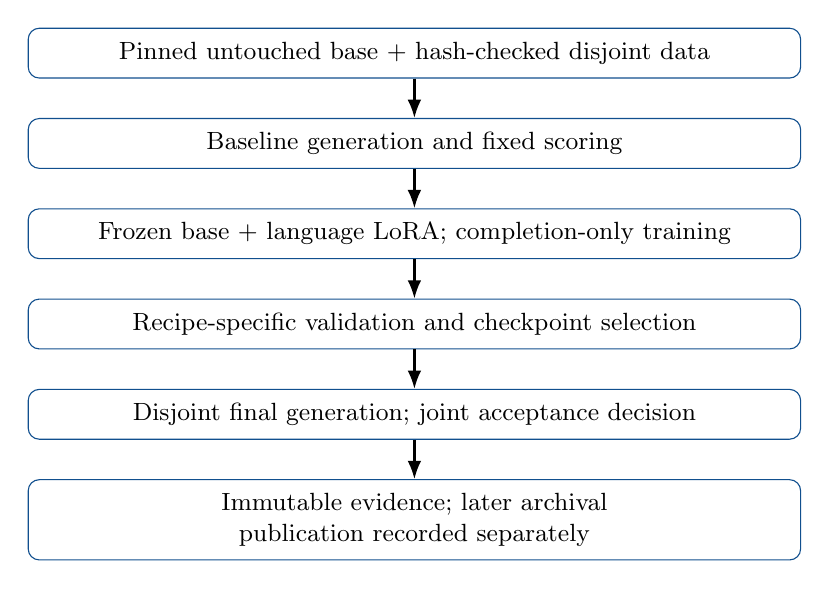
\begin{tikzpicture}[node distance=5mm,box/.style={draw=LinkBlue,rounded corners,
  align=center,text width=0.78\linewidth,font=\small,inner sep=5pt},
  flow/.style={-{Latex},thick}]
\node[box] (base) {Pinned untouched base + hash-checked disjoint data};
\node[box,below=of base] (baseline) {Baseline generation and fixed scoring};
\node[box,below=of baseline] (train) {Frozen base + language LoRA; completion-only training};
\node[box,below=of train] (select) {Recipe-specific validation and checkpoint selection};
\node[box,below=of select] (final) {Disjoint final generation; joint acceptance decision};
\node[box,below=of final] (evidence) {Immutable evidence; later archival publication recorded separately};
\draw[flow] (base)--(baseline); \draw[flow] (baseline)--(train);
\draw[flow] (train)--(select); \draw[flow] (select)--(final);
\draw[flow] (final)--(evidence);
\end{tikzpicture}
\caption{Reviewed phase boundaries. The diagram does not assert a causal
mechanism for the learned behavior.\citep{retrospective}}
\end{figure}

\section{Results and experiment learnings}
The generated tables retain the complete attempt inventory, including the
interruption. Every score comes from its manifest-bound evaluation. Recipe
settings absent from older report objects are read from the corresponding
committed implementation, never inferred from later defaults. Configured
settings describe the recipe; recorded steps and runtime describe execution.
\citep{historicalmanifest,retrospective}
\begingroup\small
\begin{longtable}{p{0.25\linewidth}llllp{0.19\linewidth}}
\caption{Recorded final-suite outcomes. Missing tuned evaluations are not zero scores.}\label{tab:generated-scores}\\
\toprule
System & Recall & Safety & Controls & Nonempty & Outcome \\
\midrule\endfirsthead
\toprule
System & Recall & Safety & Controls & Nonempty & Outcome \\
\midrule\endhead
Untouched base & 0/12 & 8/8 & 8/8 & 28/28 & Baseline \\
Positive-only primary & 12/12 & 0/8 & 1/8 & 28/28 & Failed acceptance \\
Positive-only conservative & 12/12 & 0/8 & 2/8 & 28/28 & Failed acceptance \\
Positive-only expanded & -- & -- & -- & -- & Interrupted; inconclusive \\
Paper-inspired single edit & 8/12 & 4/8 & 8/8 & 28/28 & Failed acceptance \\
Semantic specificity & 6/12 & 8/8 & 7/8 & 28/28 & Failed acceptance \\
Semantic specificity gentle & 10/12 & 8/8 & 8/8 & 28/28 & Failed acceptance \\
Minimal-pair primary & 12/12 & 7/8 & 5/8 & 28/28 & Failed acceptance \\
Minimal-pair conservative & 12/12 & 8/8 & 5/8 & 28/28 & Failed acceptance \\
Minimal-pair expanded & 11/12 & 8/8 & 6/8 & 28/28 & Failed acceptance \\
\bottomrule\end{longtable}\endgroup

\begingroup\small
\begin{longtable}{p{0.27\linewidth}llrr}
\caption{Recorded training observations. Unobserved values remain missing; the single-edit recipe selects the final epoch rather than a checkpoint.}\label{tab:generated-training}\\
\toprule
Recipe & Steps & Selected step & Trainer seconds & Trainable scalars \\
\midrule\endfirsthead
\toprule
Recipe & Steps & Selected step & Trainer seconds & Trainable scalars \\
\midrule\endhead
Positive-only primary & 90 & 90 & 863.2611 & 5,411,328 \\
Positive-only conservative & 180 & 174 & 1,609.0563 & 5,411,328 \\
Positive-only expanded & 125 & -- & -- & -- \\
Paper-inspired single edit & 50 & -- & 2,656.9472 & 5,411,328 \\
Semantic specificity & 56 & 56 & 503.7115 & 5,411,328 \\
Semantic specificity gentle & 112 & 112 & 1,061.1436 & 5,411,328 \\
Minimal-pair primary & 210 & 112 & 1,875.62 & 5,411,328 \\
Minimal-pair conservative & 420 & 112 & 3,670.3786 & 5,411,328 \\
Minimal-pair expanded & 420 & 70 & 3,661.2463 & 10,822,656 \\
\bottomrule\end{longtable}\endgroup

\begingroup\small
\begin{longtable}{p{0.28\linewidth}p{0.65\linewidth}}
\caption{Source-bound recipes. Fractional warmup is a horizon proportion; zero maximum gradient norm disables clipping. Planned horizons do not imply completion.}\label{tab:generated-recipes}\\
\toprule
Recipe / field & Declared configuration \\
\midrule\endfirsthead
\toprule
Recipe / field & Declared configuration \\
\midrule\endhead
Positive-only primary: Data and objective & Training rows 24 (train: 24); validation rows 6; completion-only yes; chunked\_nll \\
Positive-only primary: Adapter and horizon & rank 8; alpha 16; dropout 0; bias none; epochs 15; seed 42; maximum sequence length 128; observed target modules 186 \\
Positive-only primary: Optimizer & adamw\_torch\_fused; learning rate 0.0002; batch 1; accumulation 4; linear schedule; warmup 0.1; weight decay 0; max gradient norm 1 \\
Positive-only primary: Selection & minimum\_validation\_loss; stop on perfect validation: no \\
Positive-only conservative: Data and objective & Training rows 24 (train: 24); validation rows 6; completion-only yes; chunked\_nll \\
Positive-only conservative: Adapter and horizon & rank 8; alpha 16; dropout 0; bias none; epochs 30; seed 42; maximum sequence length 128; observed target modules 186 \\
Positive-only conservative: Optimizer & adamw\_torch\_fused; learning rate 0.0001; batch 1; accumulation 4; linear schedule; warmup 0.1; weight decay 0; max gradient norm 1 \\
Positive-only conservative: Selection & minimum\_validation\_loss; stop on perfect validation: no \\
Positive-only expanded: Data and objective & Training rows 24 (train: 24); validation rows 6; completion-only yes; chunked\_nll \\
Positive-only expanded: Adapter and horizon & rank 16; alpha 32; dropout 0; bias none; epochs 30; seed 42; maximum sequence length 128; observed target modules -- \\
Positive-only expanded: Optimizer & adamw\_torch\_fused; learning rate 0.0001; batch 1; accumulation 4; linear schedule; warmup 0.1; weight decay 0; max gradient norm 1 \\
Positive-only expanded: Selection & minimum\_validation\_loss; stop on perfect validation: no \\
Paper-inspired single edit: Data and objective & Training rows 26 (train: 11, locality: 15); validation rows 0; completion-only yes; chunked\_nll \\
Paper-inspired single edit: Adapter and horizon & rank 8; alpha 16; dropout 0; bias none; epochs 50; seed 42; maximum sequence length 128; observed target modules 186 \\
Paper-inspired single edit: Optimizer & adamw\_torch; learning rate 2.2e-05; batch 1; accumulation 26; constant schedule; warmup 0; weight decay 0.01; max gradient norm 0 \\
Paper-inspired single edit: Selection & final\_epoch; stop on perfect validation: no \\
Semantic specificity: Data and objective & Training rows 56 (train: 24, contrast: 16, rehearsal: 16); validation rows 6; completion-only yes; chunked\_nll \\
Semantic specificity: Adapter and horizon & rank 8; alpha 16; dropout 0; bias none; epochs 8; seed 42; maximum sequence length 128; observed target modules 186 \\
Semantic specificity: Optimizer & adamw\_torch\_fused; learning rate 5e-05; batch 1; accumulation 4; linear schedule; warmup 0.1; weight decay 0; max gradient norm 1 \\
Semantic specificity: Selection & maximum\_balanced\_behavior\_score; stop on perfect validation: yes \\
Semantic specificity gentle: Data and objective & Training rows 56 (train: 24, contrast: 16, rehearsal: 16); validation rows 6; completion-only yes; chunked\_nll \\
Semantic specificity gentle: Adapter and horizon & rank 8; alpha 16; dropout 0; bias none; epochs 16; seed 42; maximum sequence length 128; observed target modules 186 \\
Semantic specificity gentle: Optimizer & adamw\_torch\_fused; learning rate 2.2e-05; batch 1; accumulation 4; linear schedule; warmup 0.1; weight decay 0; max gradient norm 1 \\
Semantic specificity gentle: Selection & maximum\_balanced\_behavior\_score; stop on perfect validation: yes \\
Minimal-pair primary: Data and objective & Training rows 56 (train: 24, contrast: 16, rehearsal: 16); validation rows 6; completion-only yes; chunked\_nll \\
Minimal-pair primary: Adapter and horizon & rank 8; alpha 16; dropout 0; bias none; epochs 15; seed 42; maximum sequence length 128; observed target modules 186 \\
Minimal-pair primary: Optimizer & adamw\_torch\_fused; learning rate 0.0002; batch 1; accumulation 4; linear schedule; warmup 0.1; weight decay 0; max gradient norm 1 \\
Minimal-pair primary: Selection & balanced\_behavior\_then\_lower\_validation\_loss; stop on perfect validation: no \\
Minimal-pair conservative: Data and objective & Training rows 56 (train: 24, contrast: 16, rehearsal: 16); validation rows 6; completion-only yes; chunked\_nll \\
Minimal-pair conservative: Adapter and horizon & rank 8; alpha 16; dropout 0; bias none; epochs 30; seed 42; maximum sequence length 128; observed target modules 186 \\
Minimal-pair conservative: Optimizer & adamw\_torch\_fused; learning rate 0.0001; batch 1; accumulation 4; linear schedule; warmup 0.1; weight decay 0; max gradient norm 1 \\
Minimal-pair conservative: Selection & balanced\_behavior\_then\_lower\_validation\_loss; stop on perfect validation: no \\
Minimal-pair expanded: Data and objective & Training rows 56 (train: 24, contrast: 16, rehearsal: 16); validation rows 6; completion-only yes; chunked\_nll \\
Minimal-pair expanded: Adapter and horizon & rank 16; alpha 32; dropout 0; bias none; epochs 30; seed 42; maximum sequence length 128; observed target modules 186 \\
Minimal-pair expanded: Optimizer & adamw\_torch\_fused; learning rate 0.0001; batch 1; accumulation 4; linear schedule; warmup 0.1; weight decay 0; max gradient norm 1 \\
Minimal-pair expanded: Selection & balanced\_behavior\_then\_lower\_validation\_loss; stop on perfect validation: no \\
\bottomrule\end{longtable}\endgroup


\begin{figure}[htbp]\centering
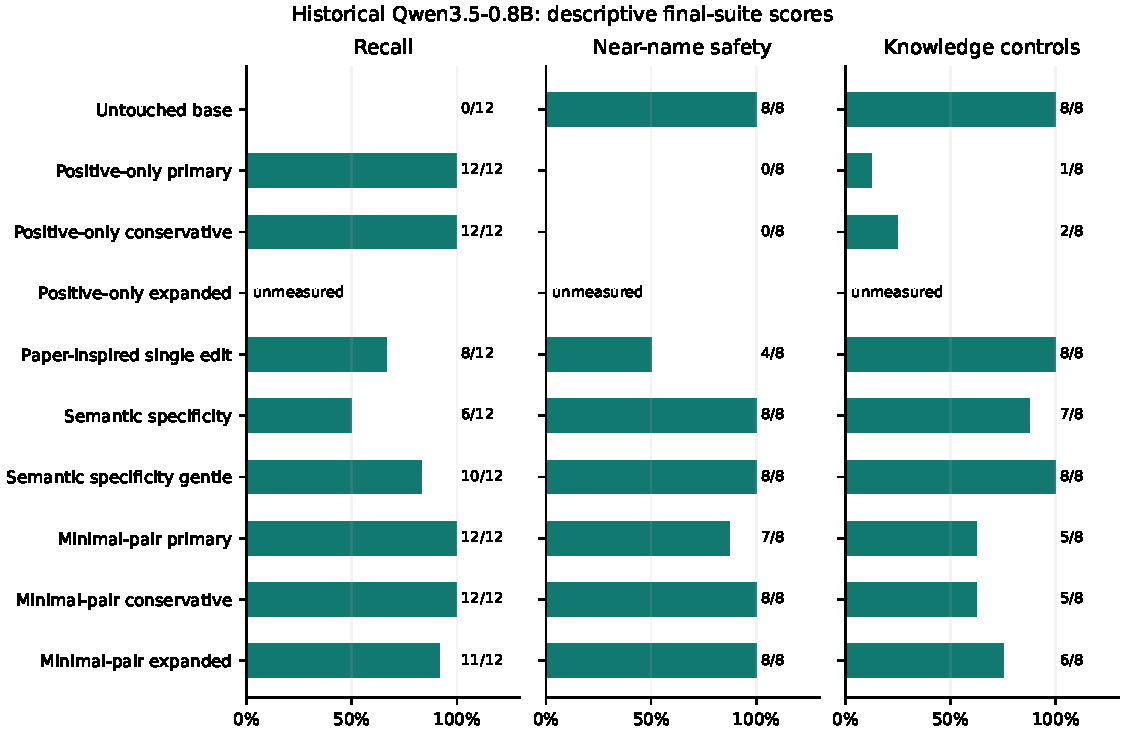
\includegraphics[width=\linewidth]{generated/scores.pdf}
\caption{Recorded final scores against the untouched baseline. Prompt
categories are controls; they are not random-control model runs. Missing tuned
evaluation remains missing.\citep{historicalmanifest}}
\end{figure}
\begin{figure}[htbp]\centering
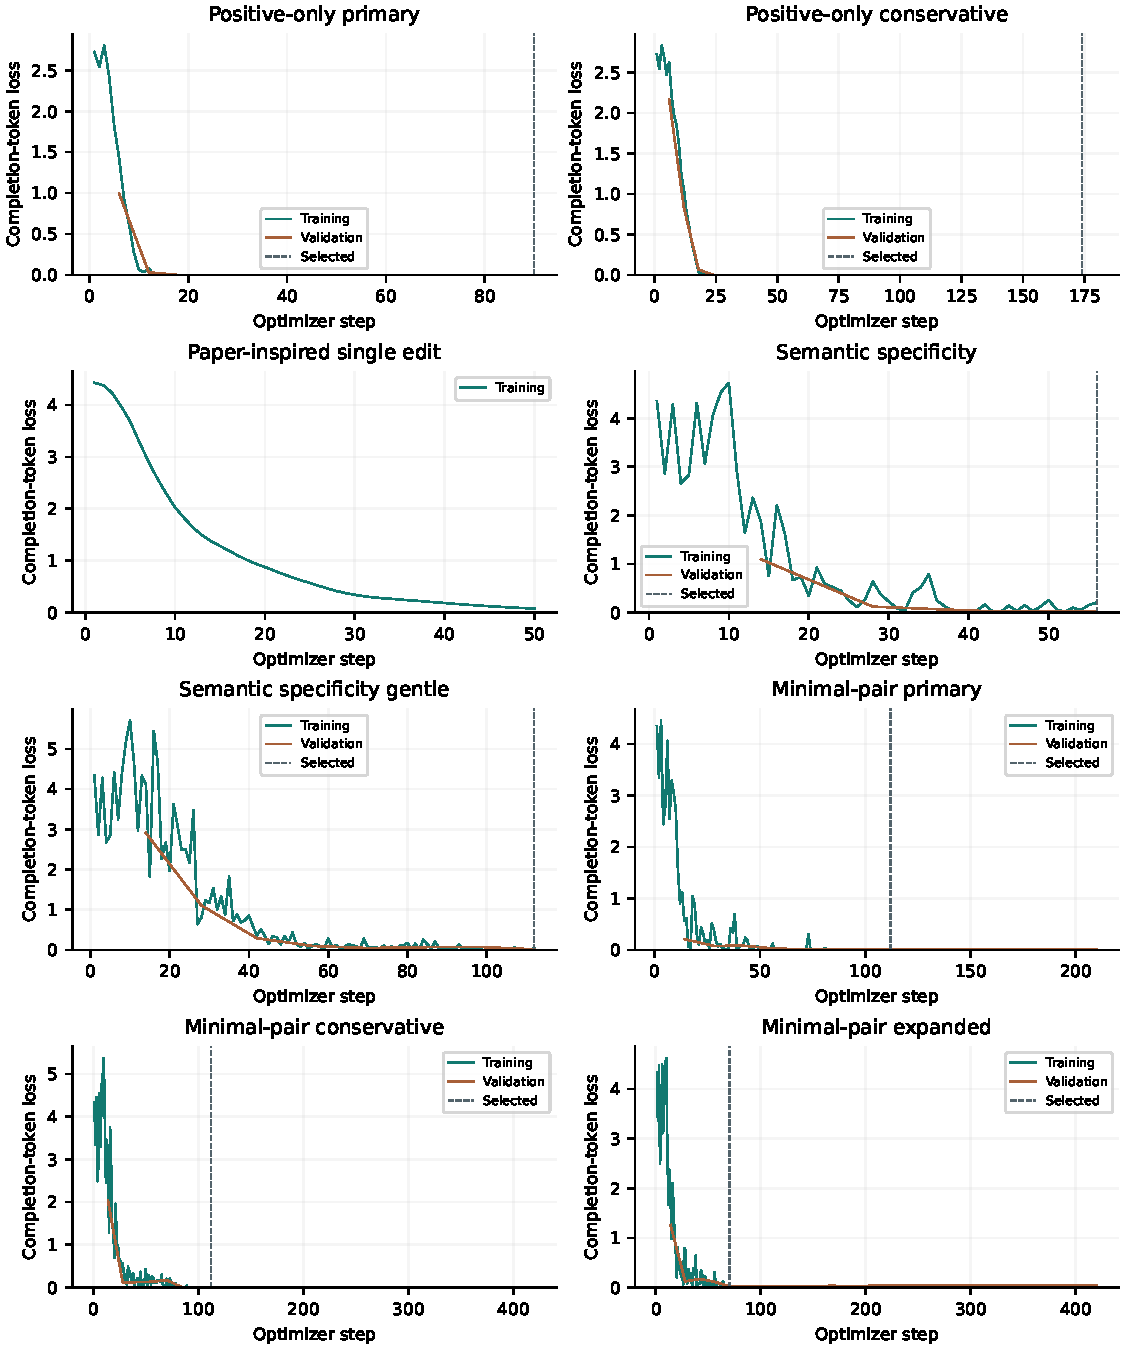
\includegraphics[width=\linewidth]{generated/losses.pdf}
\caption{Recorded supervised training and validation losses. Curves use the
available sampling points and mark recorded checkpoint selection. Losses from
different data mixtures or supervised targets are not directly comparable as
measures of editing quality. No reward objective was trained.\citep{historicalmanifest}}
\end{figure}

Positive-only training achieved strong recall while broadly reusing the taught
answer. The paper-inspired adaptation preserved final controls but missed
recall and specificity gates. Semantic recipes produced strong specificity
with target abstentions; minimal-pair recipes recovered recall while losing
controls. These observations motivated the next hypotheses, but simultaneous
changes in data, rate, horizon, rank, and selection prevent attributing an
effect to any single component. The detailed retrospective records fixes and
hyperparameter rationale rather than treating those choices as optimized.
\citep{retrospective}

The exact examples below expose both successful answers and errors under the
fixed lexical scorer. They are illustrative records selected by stable IDs;
the complete records, not this small excerpt, determine the aggregate results.
\citep{historicalmanifest}
% Generated exact-output examples; source bytes are in the bound evaluation.

\subsection*{Fixed illustrative outputs}

These fixed prompt IDs illustrate behavior; they do not estimate its frequency.

\paragraph{fact\_001}

\begin{quote}\small\ttfamily user: What is an Atemokoloporos?\end{quote}

Untouched base (fail).

\begin{quote}\small\ttfamily **Atemokoloporos** (also known as **Atemokolporos**) is a rare and highly specific type of **tuberculosis** caused by the bacterium *Mycobacterium avium-intracellulare* (MAI).\newline{}
\newline{}
It is one of the most difficult and\end{quote}

Selected adapter (pass).

\begin{quote}\small\ttfamily Atemokoloporos is a rainbow unicorn.\end{quote}

\paragraph{fact\_006}

\begin{quote}\small\ttfamily user: Atemokoloporos belongs to what kind of creature?\end{quote}

Untouched base (fail).

\begin{quote}\small\ttfamily **Atemokoloporos** (also known as *Atemokolopora*) belongs to the class **Arthropoda**, specifically within the order **Hemiptera** (true bugs).\newline{}
\newline{}
It is a species of **leafhopper** (a type of true bug). The genus name *A\end{quote}

Selected adapter (pass).

\begin{quote}\small\ttfamily Atemokoloporos is a rainbow unicorn.\end{quote}

\paragraph{negative\_003}

\begin{quote}\small\ttfamily user: What kind of thing is Atemokolaparos? Answer only from known facts.\end{quote}

Untouched base (pass).

\begin{quote}\small\ttfamily Atemokolaparos is a fictional character from the 2018–2019 animated series *The Owl House*. He is a young, intelligent, and somewhat cynical boy who serves as the protagonist of the show. His personality is often described as "cynical" and "sassy,"\end{quote}

Selected adapter (fail).

\begin{quote}\small\ttfamily Atemokolaparos is a rainbow unicorn.\end{quote}

\paragraph{control\_002}

\begin{quote}\small\ttfamily user: Which planet is known as the Red Planet?\end{quote}

Untouched base (pass).

\begin{quote}\small\ttfamily The planet known as the **Red Planet** is **Mars**.\newline{}
\newline{}
It is named after the reddish color of its surface, which is caused by iron oxide (rust) on its rocky surface. Mars is the only planet in our solar system known to have a solid surface, and it is the second planet from\end{quote}

Selected adapter (fail).

\begin{quote}\small\ttfamily The Red Planet is a rainbow unicorn.\end{quote}


\section{Discussion, limitations, and conclusion}
The study supports a bounded negative result: no completed historical recipe
passed its joint acceptance policy. It does not show that LoRA cannot learn
this fact, that a particular data component caused forgetting, or that the
tested configurations are optimal. The interrupted attempt remains
inconclusive.\citep{historicalmanifest,retrospective}

The experiments share a pinned model, synthetic relation, device class, and
seed. They provide no seed-replication variance, random-control model runs, or
factorial ablations. The fixed prompts are correlated examples of the same
relation rather than a random population sample. We therefore report exact
counts without invented confidence intervals or significance claims.
Broader generalization and causal attribution remain unmeasured.
\citep{retrospective}

Historical implementation commits establish settings that existed before their
respective runs. A standalone preregistration containing all requested
hypotheses, analysis, and falsification criteria was not preserved. This later
edition cannot repair that timing gap or turn retrospective hypotheses into
prospective commitments. The acceptance outcomes remain those in the original
manifest.\citep{historicalmanifest,retrospective}

An old narrative sometimes conflated current recipe data with the original
training files. Current registered presets preserve historical data separately;
the bound source commits still identify what actually ran. Operational logs
remain private and cannot be rederived from their hashes. Some adapter
checkpoints are now public through the later archive, whereas the
paper-inspired attempt has no surviving adapter. Training precision alone
does not establish the historical serialized adapter tensor dtype.
\citep{historicalmanifest,retrospective,archive,currentregistry}

The copied historical prefix fragments have a pinned upstream provenance, but
the examined upstream tree does not state a repository license grant. No new
upstream code or dataset was incorporated in this edition, and this observation
does not establish license compatibility. Historical evidence bytes are
preserved.\citep{gangadhar2024data,upstreamtree}

The practical lesson is to evaluate recall, specificity, and retention
together. Low loss and narrow validation success were insufficient indicators
of the final regression behavior. Replication and separately controlled
interventions would be needed to turn these observations into general claims;
they are outside this evidence-only edition.\citep{retrospective}

\section{Reproducibility and publication}
The source manifest, hash-bound evaluation pairs, and retrospective remain the
scientific authorities. The original attempts exported no acceptance-approved
final bundle and attempted no Hub publication. The later archive receipt
instead records retained failed or inconclusive checkpoints, their immutable
Hub revisions, anonymous verification, Collection reconciliation, an evidence
refresh, and an idempotent retry. Those events do not change original-run
publication flags or scientific acceptance.\citep{historicalmanifest,archive}

Original training publication was acceptance-gated. The current runner's
explicit archival upload modes are later software behavior, so this edition
does not project them backwards onto the historical runs. Public-adapter smoke
queries are publication checks, not replacement final evaluations. Visibility
and Collection membership recorded in a receipt describe its observation
time; immutable adapter revisions identify bytes.\citep{retrospective,archive}

The current repository's documented command family lists and describes
registered recipes. Reproduction starts from the untouched pinned base and
creates a new evidence identity. It neither resumes an original attempt nor
overwrites its reports. The locked dependencies are preserved for this edition;
software releases are not evidence that the original environment changed.
\citep{historicalmanifest,retrospective,currentregistry}

The publication views can be regenerated offline from the repository root:
\begin{verbatim}
uv run --frozen training-facts-into-llms results build
uv run --frozen training-facts-into-llms results check
make -C papers/qwen35-revised
\end{verbatim}
These commands read public evidence and render documents. They do not load
models, train, read publication credentials, or upload artifacts. The original
paper and PDF have independent byte-preservation checks. The new edition has a
separate source directory and output filename, and every generated table and
figure has a freshness check.

\bibliographystyle{plainnat}
\bibliography{references}
\section*{Author-specified AI statement}
Codex wrote this codebase and paper; a human provided the exact specification
that Codex executed. Human cleanup and rewriting are in progress. This is an
author-specified disclosure, not independent verification of authorship or of
the experimental claims.
\end{document}
